\chapter{s--d-model}
\section{Introduction}
Our model consists of two parts. The first part are the conducting electrons who's Hamiltonian is given by a tight-binding model. These conducting electrons can scatter of impurities in the material leading to having a finite momentum life-time. At the same time the spin of the electrons are coupled to its momentum through spin-orbit interactions, making it possible to transfer this angular momentum to the crystal lattice. The second part is the (anti)ferromagnet which we describe using a Heisenberg model in a classical limit, meaning we replace the spin-operators with vectors. In order to transfer angular momentum between localized and itinerant electrons, we therefore need to introduce a parameter that couples the spin and magnetic moment locally. This allows us to directly relate the relaxation of the momentum of itinerant electrons to the relaxation of angular momentum of the localized electrons. This momentum relaxation is at the heart of quantum transport theory. This model has much in comparison with the s--d model, used for example in the Kondo effect \cite{kondo}, where localized $d$ electrons are coupled to itinerant $s$ electrons. In the literature therefore our model is often called s--d, or s--d-like, and the parameter that couples the spins of localized and itenerant electrons is called an s--d-like exchange interaction. 

\section{Classical equations of motion on magnetization}
The Hamiltonian describing the localized and intenerant electrons is given by
\begin{multline}
    \hat{H}
        = \sum_{\mathclap{\{i,j\}\in\text{n.n.}}}\,\Big(\frac{J_{\text{ex}}}{n}\hat{\bb{S}}_i\cdot\hat{\bb{S}}_j - \frac{K}{2n}\hat{\bb{S}}_{z,i}\cdot\hat{\bb{S}}_{z,j}-t \hat{c}_i^\dagger\hat{c}_j\\
        -\lambda i c_i^\dagger \bb{u}_{ij}\cdot\bb{\sigma}\hat{c}_j\Big)+\sum_i \hslash\gamma_0\bb{H}_\text{ext}\cdot\hat{\bb{S}}_i-\Delta_\text{sd}\hat{\bb{S}}_i\cdot\hat{c}_i^\dagger\bb{\sigma}\hat{c}_i,
    \label{intro:eq:Hm}
\end{multline}
with the Heisenberg exchange energy $J_{\text{ex}}$, anisotropy constant $K$, s--d-like exchange energy $J_{\text{sd}}$, creation operators for itinerant electrons and localized spins $\hat{c}^\dagger_l$ and $\hat{S}$ respectively, Pauli-matrices $\bb{\sigma}$, external magnetic field $\bb{H}_\text{ext}$, gyromagnetic ratio $\gamma_0=|\gamma_0|$, hopping parameter $t$ and Rashba-spin-orbit $\lambda$, and $\bb{u}_{ij}$ is a vector that connects nearest neighbors at sites $i$ and $j$.  The first sum is taken over nearest neighbor sites. Note that the constant $K$ is inserted here phenomenologically, but can be computed as done later in Chapter~\ref{?} for a honeycomb antiferromagnet.

To describe the full dynamics of the system we assume that the expectation value of the localized spins move on a much larger time-scale than the spin-polarization of the conducting electrons. This allows us to decouple the system in two parts. We first derive equations of motion for the localized spins in a classical, mean-field approach by using only the expectation value of conducting electrons spin-polarization. Second, the spin-polarization of the conducting electrons is computed microscopically using linear response theory in response to electric currents and time-derivative of magnetizations, where the localized spins enter as classical fields. 

The mean-field approach simply constitutes the replacement
\begin{equation}
    \sum_{\mathclap{\{ij\}\in\text{n.n.}}} \bb{S}_i\cdot\bb{S}_j\rightarrow n\langle\bb{S}_j\rangle\cdot\sum_i \bb{S}_i
\end{equation}
with $n \langle \bb{S}_j\rangle$ the effective field produced by the $n$ nearest neighbors felt by $\bb{S}_i$. When $J_\text{ex}<0$, the spins favour parallel alignment and the energy can be written as
\begin{multline}
    E = \sum_{i} \Big(\mu_0 \hat{\bb{S}}_i\cdot \bb{H}_{\text{ext}}
    - K(\hat{S}_{z,i})^2)
    -J_{\text{sd}}\big(\bb{S}_i\cdot\bb{s}\big)
        \Big)
        \label{intro:eq:E1}
\end{multline}
where we introduced the spin polarization density $\bb{s} = \mathcal{A}^{-1}\langle \hat{c}^\dagger \bb{\sigma}\hat{c}\rangle$ (with unit cell area $\mathcal{A}$). In the case when $J_\text{ex}>0$ the spins favor antiparallel alignment and the energy can be written as
\begin{multline}
    E = \sum_{i} \Big(J_{\text{ex}}\bb{S}^\text{A}_i\cdot\bb{S}^\text{B}_i 
    - K((\hat{S}_{z,i}^\text{A})^2+(\hat{S}_{z,i}^\text{B})^2)
    -J_{\text{sd}}\big(\bb{S}^\text{A}_i\cdot\bb{s}^\text{A}+\bb{S}^\text{B}_i\cdot\bb{s}^\text{B}\big)
        \Big)
        \label{intro:eq:E2}
\end{multline}
where we introduced the spin polarization density $\bb{s}^\text{A(B)} = \mathcal{A}^{-1}\langle \hat{c}^\dagger \bb{\sigma}\hat{c}\rangle$ (with unit cell area $\mathcal{A}$). 

The equations of motion is given by $\partial_t \bb{S}_i = \{E,\bb{S}_i\}_p$, where $\{\cdots\}_p$ is the Poisson bracket. For angular momenta we simply have $\{\hslash \bb{S}_i,\hslash \bb{S}_j\}_p=\hslash \bb{S}_i\times\bb{S}_j$. With these considerations we find the following equations of motion for a ferromagnet
\begin{align}
	\hslash \partial_t \bb{S} &= \bb{S}\times\big(-\hslash\gamma_0\bb{H}_\text{ext}-KS_z+\Delta_\text{sd}\bb{s}\big)
	\label{intro:eq:S1}
\end{align}
and the following for an antiferromagnet
\begin{align}
   \hslash \partial_t \bb{S}^\text{A} &= \bb{S}^\text{A}\times\big( -\hslash\gamma_0\bb{H}_\text{ext}-KS^A_z-J_\text{ex}\bb{S}^\text{B}+J_\text{sd}\bb{s}^\text{A}\big)\\
      \hslash \partial_t \bb{S}^\text{B} &= \bb{S}^\text{B}\times\big( -\hslash\gamma_0\bb{H}_\text{ext}-KS^B_z-J_\text{ex}\bb{S}^\text{A}+J_\text{sd}\bb{s}^\text{B}\big).
      \label{intro:eq:S2}
\end{align}

The same equations of motion can be obtained by first using Heisenberg's equations of motion $i \partial_t \hat{S}_\alpha = [H,\hat{S}_\alpha]$ (where $\alpha=x,y,z$) and the commutation relations for spin-operators $[\hat{S}_x, \hat{S}_y]=i\hat{S}_z$ on Eq~(\ref{intro:eq:Hm}), and then taking the classical limit $\hat{\bb{S}}\rightarrow \bb{S}$. 

As is common practice, the magnetization in the ferromagnet is expressed in terms of a unit vector $\bb{m} = -\bb{S}/|\bb{S}|$ and for an antiferromagnet we introduce the magnetization $\bb{m}$ and staggered magnetization $\bb{n}$ as
\begin{align}
 	\bb{n}=-1/2(\bb{S}^\text{A}/|\bb{S}^\text{A}|-\bb{S}^\text{B}/|\bb{S}^\text{B}|)
 	\bb{m}=-1/2(\bb{S}^\text{A}/|\bb{S}^\text{A}|+\bb{S}^\text{B}/|\bb{S}^\text{B}|).
 \end{align} 
Note that the minus in front of the definitions of $\bb{n}$ and $\bb{m}$ are there because for electrons their magnetic moment is directed in opposite direction of their spin angular moment. Furthermore, although we use the same notation $\bb{m}$ for the magnetization in a ferro and anti-ferromagnet, it is only a unit-vector in the former case and not the latter. 

The equations of motion for an antiferromagnet are often expressed in terms of 
next we write $\bb{S}^\text{A(B)}=-|S|\bb{n}^\text{A(B)}$, with $|S|$ the total localized spin and unit vector $\bb{n}$ pointing in the magnetization direction. From now on we set $\hslash=1$ for convenience. Furthermore we introduce new quantities: average magnetization $\bb{m}=1/2(\bb{n}^\text{A}+\bb{n}^\text{B})$ and staggered magnetization (Neel vector) $\bb{l}=1/2(\bb{n}^\text{A}-\bb{n}^\text{B})$, and similarly average(staggered) spin-density $\bb{s}^\pm=\bb{s}^\text{A}\pm\bb{s}^\text{B}$, so that equations of motion on $\bb{m}$ and $\bb{l}$ read:
\begin{align}
    \partial_t \bb{m} &= -\Delta_\text{sd}(\bb{m}\times\bb{s}^++\bb{l}\times\bb{s}^-)\label{intro:eq:dm}\\
        \partial_t \bb{l} &=-2J_\text{ex}\bb{l}\times\bb{m} -\Delta_\text{sd}(\bb{m}\times\bb{s}^-+\bb{l}\times\bb{s}^+),\label{intro:eq:dl}
\end{align}
the external field is absorbed into $\bb{s}^+$. The term $\bb{m}\times\bb{s}^-$ is generally to as Neel torque. Note that contrary to ferromagnets, the dynamics of antiferromagnets contains a term $\bb{l}\times\bb{m}$ that is proportional to the exchange energy. 

In order to compute a spin-torque, all we need to do is compute the spin-density of the conducting electrons, which is done using linear response theory. 
The dynamics of the magnetization vector in ferromagnets and antiferromagnets are determined by spin-torques. These torques can be divided into two groups: field-like and damping-like. For antiferromagnets each group can be subdivided into two: staggered and non-staggered. In a two-dimensional ferromagnet with spin-orbit of Rashba type, the equations of motion are often written phenomenologically as
\begin{equation}
    \partial_t \bb{n} = c_1 \bb{n}\times (\hat{\bb{z}}\times\bb{j}) + c_2 \bb{n}\times\big(\bb{n}\times (\hat{\bb{z}}\times{j})\big) + \alpha \bb{n}\times \partial_t \bb{n},
\end{equation}
where the terms proportional to $c_1$ and $c_2$ are torques that are induced by injecting an electric current $\bb{j}$ and the term proportional to $\alpha$ describes the rate of dissipation of angular momentum and is called Gilbert damping. The field-like and damping-like torques can be identified as those that are respectively even and odd under time-reversal (i.e. changing the signs of $\bb{n}$, $\bb{j}$ and $t$). Distinguising between field-like and damping-like torques helps us understand more the dynamics of $\bb{n}$. For example, if the damping-like torques are absent one will only observe a simple precession of the magnetization vector around $\hat{\bb{z}}\times\bb{j}$. Damping-like torques allow for the dissipation of angular momentum so that over time the magnezation vector will be parallel to $\hat{\bb{z}}\times\bb{j}$. The dynamics induced by both field-like and damping-like torques are illustrated in Figure~\ref{fig:dynamics}. Note that we can change the sign of the damping-like torque by changing the direction of the electric current. If this current-induced damping-like torque overcomes the Gilbert damping one can even reverse the magnetization direction. In such a way one can construct a magnetic memory that stores a "0" or a "1" corresponding to two magnetization directions. This type of switching is illustrated in Figure~\ref{fig:switching}. The switching rate is determined by the strength of the damping-like torque which is proportional to Rashba spin-orbit coupling. {\color{blue} [some numbers for various materials. probably all less than 1eV].} It is then no surprise that putting a magnetic layer on top of a heavy metal will enhance its magnetic switching abilities. 

In an antiferromagnet however, the magnetization dynamics is more complicated. The magnetizations on two sublattices are aligned opposite to each other 




The misalignment between the spin of the conducting electrons and the direction of the magnetic moment of localized electrons induces a spin-torque that enter the equations of motion of the magnetization vector. In order to see this let us first consider the total energy $H$ of the magnetic system
\begin{equation}
    H_M = \int \mathrm{d}\bb{r}\, \Delta_\text{sd} \bb{n}\cdot\bb{s}
\end{equation}
The equations of motion can be derived by either writing the magnetic moments as quantum spins $\hat{S}$ and use Heisenberg's equation of motion $\partial_t \hat{S} = i\hbar[H, \hat{S}]$, by poisson brackets $\{H,S\}_{p}$ or by calculating the effect field. We easily obtain
\begin{equation}
    \partial_t \bb{n} = \Delta_\text{sd}\bb{n}\times\bb{s}.
\end{equation}
In this thesis we focus on spin-densities that are in response to currents and to time-derivatives of magnetization. One example would be
\begin{equation}
    \partial_t \bb{n} = \beta \bb{n}\times \hat{\bb{z}}\times\bb{j} + \beta \bb{n}\times\bb{n}\times \hat{\bb{z}}\times{j} + \alpha \bb{n}\times \partial_t \bb{n}
\end{equation}
It is convenient to decompose current-induced torques in terms that are even under time-reversal (proportional to $\beta$) and in terms that are odd (proportional to $\beta'$), which are often called field-like and damping-like torques. The field-like torques are observed as a simple precession of $\bb{n}$ around $\bb{j}$, whereas the damping-like torques are dissipative and can orient $\bb{n}$ either parallel or anti-parallel to $\bb{j}$. 


\section{other}

In order to derive the result of Eq.~(\ref{diffSOT}) and the expressions for Gilbert damping we shall adopt a particular relaxation model for both spin and orbital angular momenta of conduction electrons. For the model of Eq.~(\ref{TImodel}) those are provided by scattering on disorder potential. We choose the latter 
to be the white-noise Gaussian disorder potential that is fully characterized by a single dimensionless parameter $\alpha\ll 1$,
\be
\label{disorder}
\la V(\bb{r})\ra =0,\quad \la V(\bb{r}) V(\bb{r}') \ra = 2\pi \alpha\, (\hslash v)^2\,\delta(\bb{r}-\bb{r}'),
\e
where angular brackets stay for the averaging over the ensemble of disordered systems. 

The main building block of our analysis is the averaged Green's function in the first Born approximation
\be
\label{green}
G^{\mathrm{R}}_{\bb{p},\ep} = \frac{\ep^\textrm{R} + v(\bb{p}\times \bb{\sigma})_z-\Delta^{\textrm{R}}_z\sigma_z}
{(\ep^{\textrm{R}})^2-v^2p^2 -(\Delta^{\textrm{R}}_z)^2},
\e
where the complex parameters $\ep^\textrm{R}=\ep(1+i\pi \alpha/2)$ and  $\Delta^\textrm{R}_z= \Delta_z(1-i\pi \alpha/2)$ are found from the corresponding self-energy 
\be
\label{Sigma}
\Sigma^{\mathrm{R}}(\ep)  = 2\pi \alpha\,v^2\!\! \int\!\frac{d^2\bb{p}}{(2\pi)^2}G^\mathrm{R}_{\bb{p},\ep}, 
\e
that gives rise to  $\im \Sigma^{\mathrm{R}}= - \pi \alpha (\ep -\Delta_z \sigma_z)/2$  (strictly speaking, the RG analysis \cite{ivan} has to be applied). In the Green's function of Eq.~(\ref{green}) we shift the momentum $\bb{p}$ such that there is no direct dependence on the in-plane magnetization components $m_x$ and $m_y$. 

The next step in disorder-averaging requires the computation of vertex corrections. This means we need to replace the spin operator $\sigma_\alpha$ with a vertex corrected spin operator $\sigma_\alpha^\text{vc}$ in the ladder approximation as depicted in Fig.~\ref{fig:diagrams}(e). The crossed diagrams in Fig.~\ref{fig:diagrams}(b-d) give a contribution to the components of $\hat{K}$ of the order $\mathcal{O}(\alpha^0)$. The
only components that are modified to this order are those
corresponding to the Hall conductivity (i.e. $\sigma_{xy}$ and $\sigma_{yx}$). Details of this calculation can be found Ref.~\cite{ivan}.
%

The dressing of $\sigma_\alpha$ with a single disorder line is denoted by $\sigma_\alpha^{1\times\text{dr}}$ and is conveniently represented in the matrix form by introducing a matrix $\hat{M}$ with $16$ components $M_{\alpha\beta}$ for $\alpha,\beta=0,x,y,z$ (with $\sigma_0=1$)
    \begin{align}
       \sigma_\alpha^{1\times\text{dr}}  = 2\pi \alpha\, v^2 \int\!\frac{d^2\bb{p}}{(2\pi)^2} G^\text{A}_{\ep+\omega,\bb{p}+\bb{q}}\sigma_\alpha G^\text{R}_{\bb{p}} = \pi\alpha M_{\alpha\beta}\sigma_\beta,
        \label{chap1:eq:myseries}
    \end{align}
where the summation of the repeating index $\beta=0,x,y,z$ is assumed. Full expressions of the components of $\hat{M}$ up to second order in $\omega$ and $q$ are given by Eq.~(\ref{chap1:eq:M}a-f). 
%%%
% Fig. 2
%%%
\begin{figure}[t]
\centering
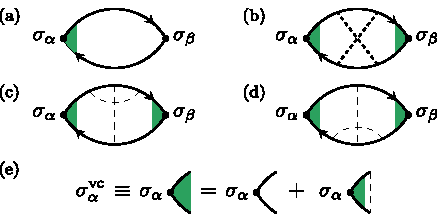
\includegraphics[]{articles/dirac_fm/fig2}
\caption{Diagrams considered in the calculation of $\hat{K}$: (a) non-crossing diagram, (b) $X$ diagram, (c-d) $\Psi$ diagrams. Green areas indicate the ladder summation (e) for the vertex correction in the non-crossing approximation \protect\cite{ivan}.}
\label{fig:diagrams}
\end{figure}

In our calculation the terms of the order of $\alpha \ln p_\textrm{cutoff}/\ep$ (where $p_\textrm{cutoff}$ is the ultraviolet momentum cut-off) is disregarded with respect to $1$. This approximation is legitimate since we assume that all model parameters $\epsilon$, $\Delta_\textrm{sd}$ and $\alpha$ are first renormalized such that $p_\textrm{cutoff} \approx \ep$.

It is, then, easy to see that the vertex-corrected spin operator is readily obtained from the geometric series of powers of $\pi\alpha \hat{M}$, 
\begin{align}
\sigma_\alpha^\text{vc} &= 
\sigma_\alpha+\pi\alpha \hat{M}_{\alpha\beta}\sigma_\beta+(\pi\alpha)^2 (\hat{M}^2)_{\alpha\beta}\sigma_\beta+\dots\nonumber\\
&=\left[1-\pi\alpha \hat{M}\right]^{-1}_{\alpha\beta}\sigma_\beta.
\end{align}
Thus, in the non-crossing approximation (illustrated in Fig.~\ref{fig:diagrams} (a)), one simply finds $\hat{K}= \hat{M}[1-\pi\alpha \hat{M}]^{-1}$. 